\section{prinsipiell løsning}
\label{sec:concept}

Ved filterdesign kan det være lurt å ha en fornuftig arbeidsgang:
\begin{enumerate}
    \item Start med spesifikasjon
    \item Velg type filter
    \item Finn nødvendig orden N
    \item Finn systemfunksjonen H(s)
    \item Realisert H(s) med tilgjenteliug teknologi
  \end{enumerate}

\subsection{Spesifikasjon}
\label{sec:spesifikasjon}
Fra problembeskrivelsen i seksjon \ref{sec:issue} blir det opplyst at dersom punktprøvingsfrekvensen er $f_s$, må båndbegrensingen være $B=\frac {f_s} {2}$ og knekkfrekvensen være $f_c \geq \frac{3}{8}f_s$. Amplituderesponsen vil da ha en form tilsvarende figur \ref{fig:02ønsketamplituderespons}.

\begin{figure}[!hbt]
	\centering
	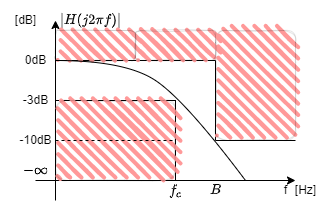
\includegraphics[scale=0.7]{./Images/02Concept/01spesifikasjon.png}
	\caption{Ønsket amplituderespons på system.}
	\label{fig:02ønsketamplituderespons}
\end{figure}

\subsection{Type filter}
\label{sec:type_filter}

For å få en amplituderespons som likner mest på figur \ref{fig:02ønsketamplituderespons} kan et Butterworth filter benyttes da den ifølge siden \cite{storr_2013_butterworth} er et analog filter som produserer den flateste amplituderesponsen, men da på bekostning av en relativt lang overgangsbånd mellom båndpass og båndstop som illustrert i figur \ref{fig:03frekvensresponsButterworth}. 

\begin{figure}[!hbt]
	\centering
	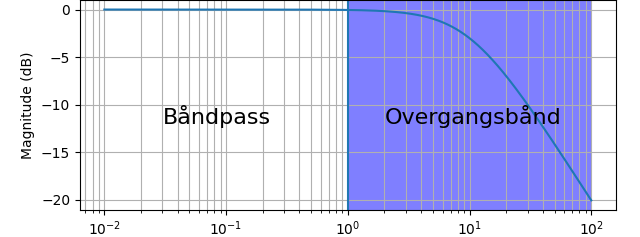
\includegraphics[scale=0.7]{./Images/02Concept/02filter.png}
	\caption{Plot av frekvensresponsen til en Butterworth lavpassfilter.}
	\label{fig:03frekvensresponsButterworth}
\end{figure}

For å få en slik filter karakteristikk kan man ta i bruk et 2. ordens Sallen-Key topologi som illustrert i figur \ref{fig:04SallenKey}.

\begin{figure}[!hbt]
	\centering
	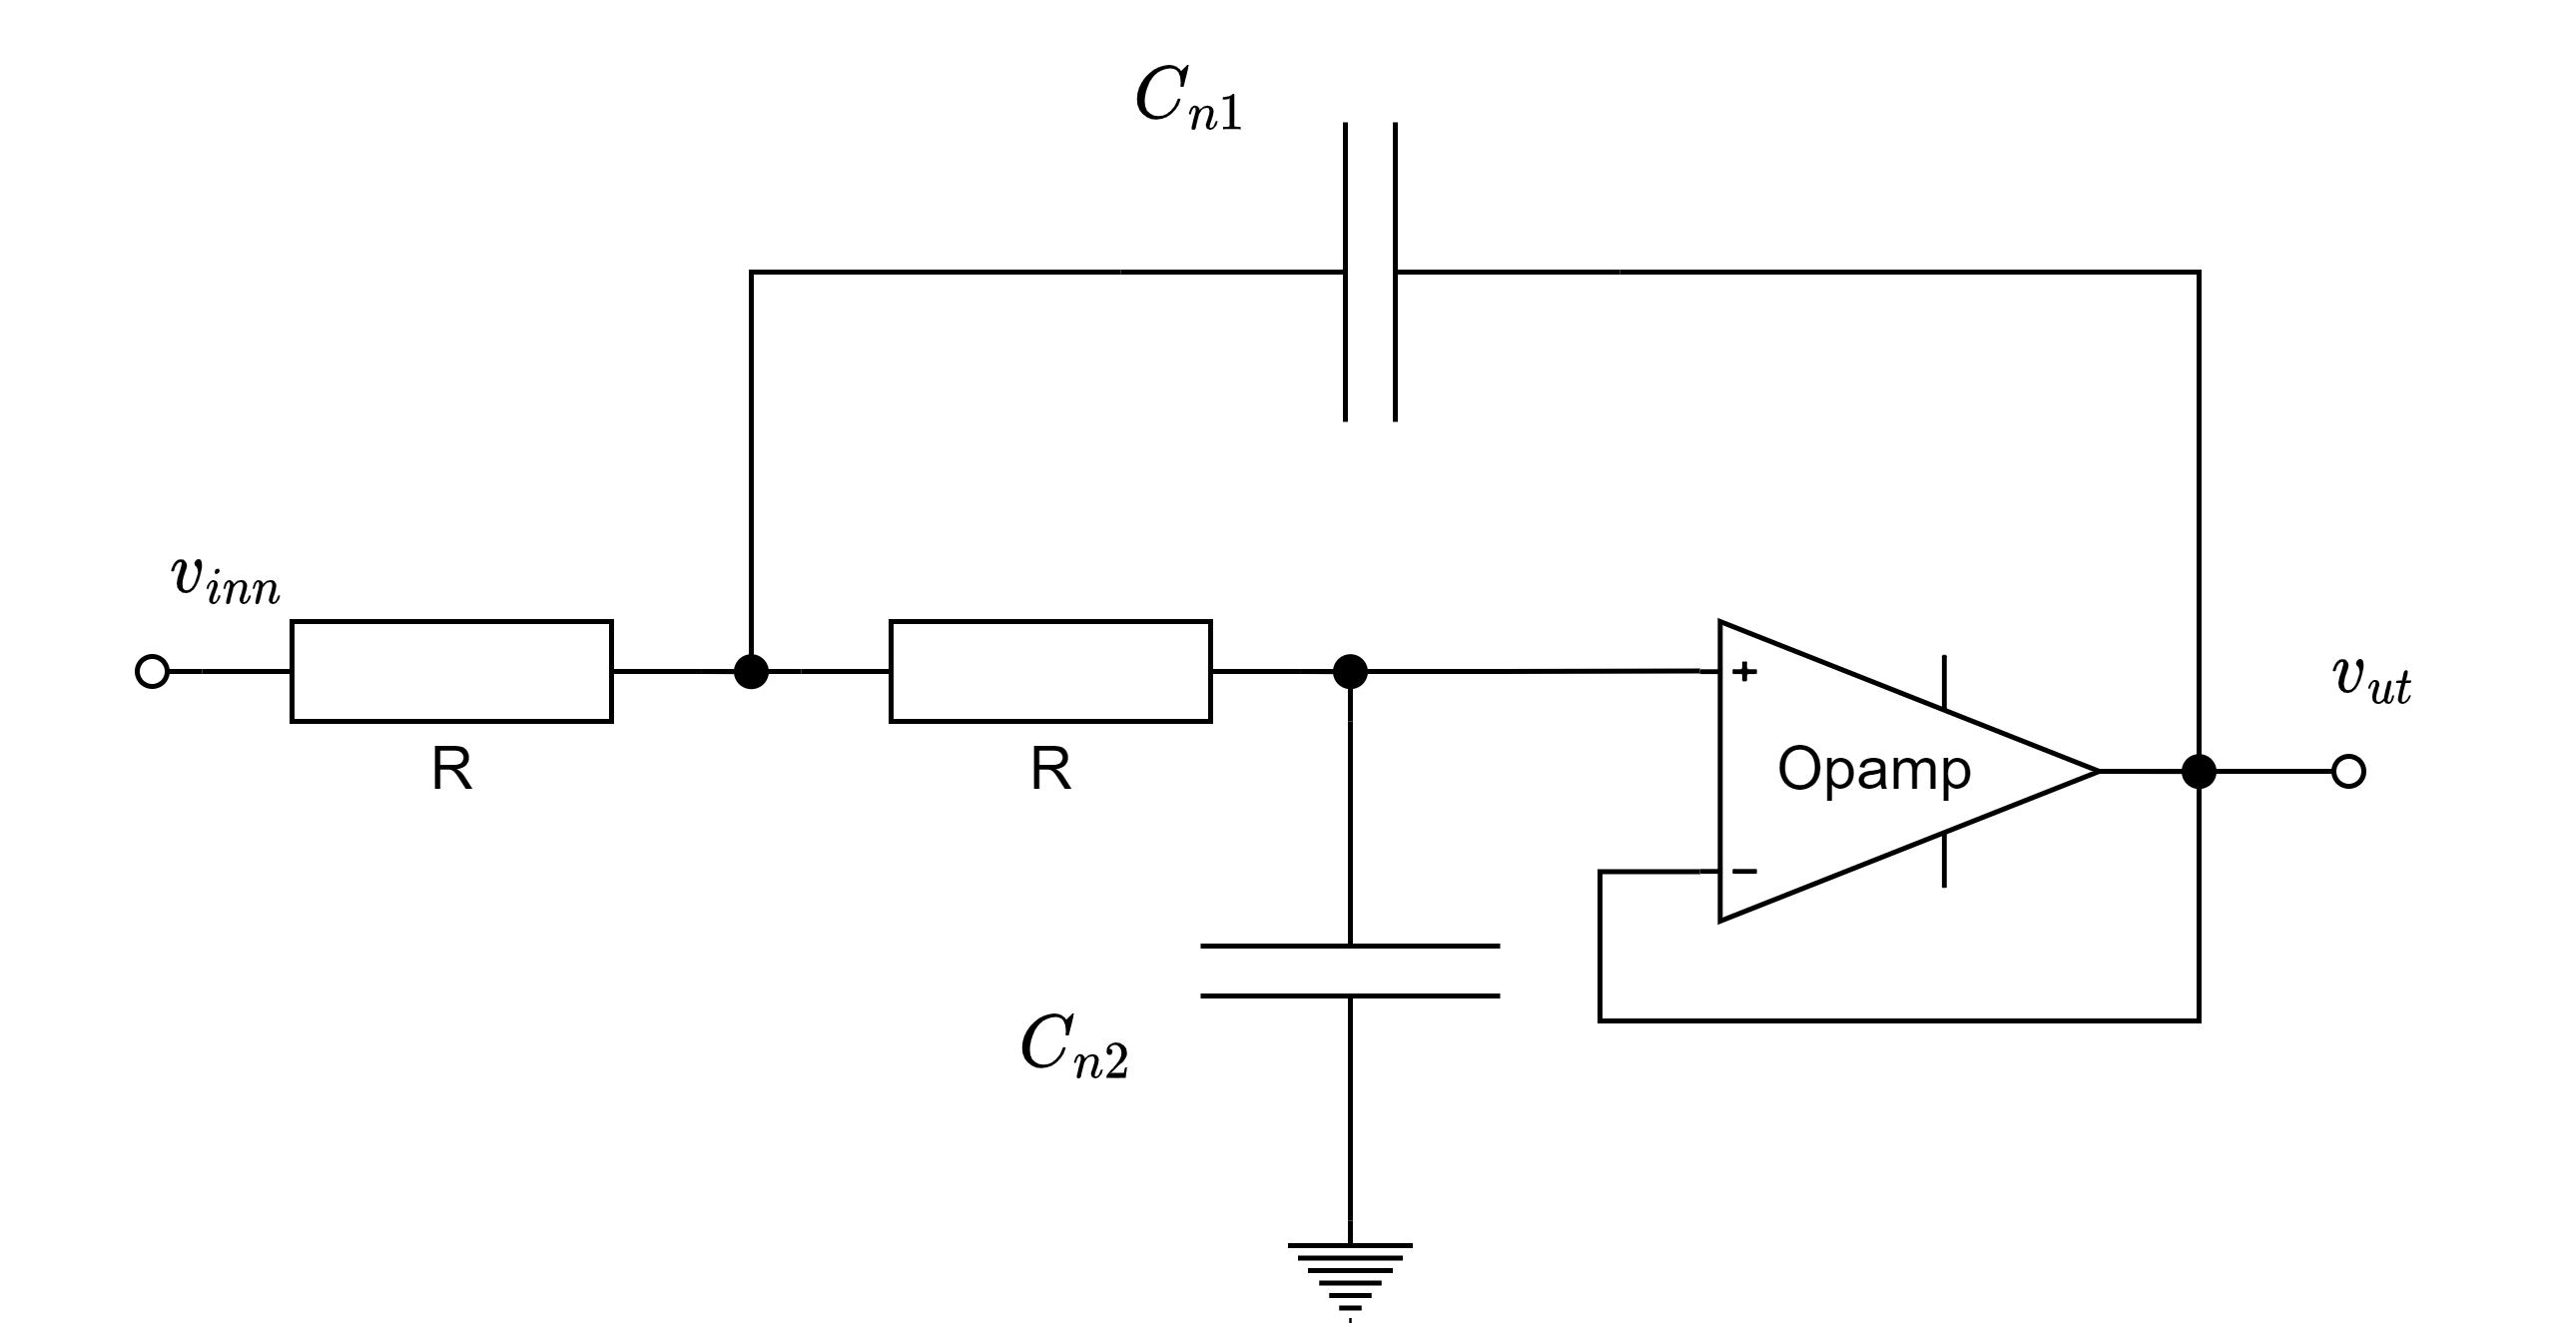
\includegraphics[scale=0.7]{./Images/02Concept/03SallenKey.png}
	\caption{Lavpassfilter med Sallen-Key topologi.}
	\label{fig:04SallenKey}
\end{figure}

\subsection{Nødvendig orden}
\label{sec:Nødvendig_orden}

Fra siden \cite{wikipediacontributors_2022_butterworth} blir det oppgitt at formelen for demping $A(\omega)$ for en $n$te-ordens Butterworth lavpasslfilter er gitt ved systemfunksjonen $H(s)$ som

\begin{equation}
	A(\omega)=|H(j2\pi f)|=\frac{1}{1+(\frac{f}{f_c})^{2n}}
	\label{eq:magnitude}
\end{equation}


Formel \ref{eq:magnitude} kan videre skrives om til

\begin{equation}
	n=\frac{1}{2}\frac{ln(A^{-2}-1)}{ln(\frac{f}{f_c})}
	\label{eq:order}
\end{equation}

Der dempingen $A$ er amplitudeforholdet, dette får man ved å bruke formelen

\begin{equation}
	A=10^{\frac{A[dB]}{20}}
	\label{eq:decibeltonone}
\end{equation}

Som man kan se på figur \ref{fig:05order} tatt fra Wikipedia \cite{wikipediacontributors_2022_butterworth} kan man se at man får et mye brattere jo høyere orden det er i filteret, men ettervert som man kommer i en høyere orden så vil også graden den blir brattere minkes. 

\begin{figure}[!hbt]
	\centering
	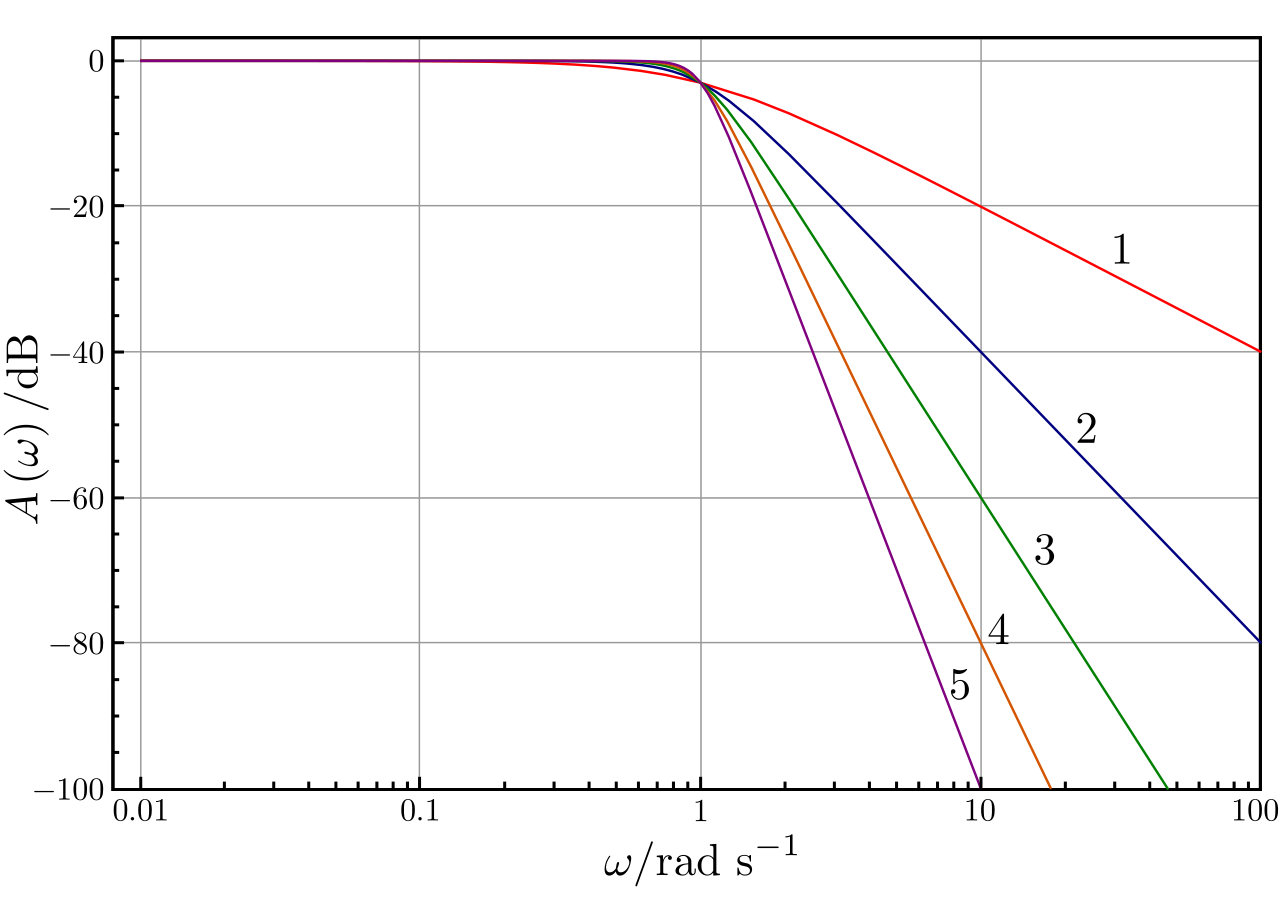
\includegraphics[scale=0.2]{./Images/02Concept/04orders.png}
	\caption{Plot med demping for et Butterworth lavpassfilter fra 1. til 5. orden med knekkfrekvens $\omega=1$.}
	\label{fig:05order}
\end{figure}

\subsection{Systemfunksjonen}
\label{sec:Systemfunksjonen}

Når man ved hjelp av formelen \ref{eq:order} kan man bruke tabellen \ref{tab:polpar} til å finne ut dempningsfaktoren $\zeta$.

\begin{table}[]
	\caption{Dempningsfaktor $\zeta$.}
	\centering
	\begin{tabular}{|l|lll|}
	\hline
	\multicolumn{1}{|c|}{} & \multicolumn{3}{c|}{Polpar i}                                         \\ \hline
	n                      & \multicolumn{1}{l|}{1}       & \multicolumn{1}{l|}{2}       & 3       \\ \hline
	1                      & \multicolumn{1}{l|}{1}       & \multicolumn{1}{l|}{}        &         \\ \hline
	2                      & \multicolumn{1}{l|}{0.70711} & \multicolumn{1}{l|}{}        &         \\ \hline
	3                      & \multicolumn{1}{l|}{1}       & \multicolumn{1}{l|}{0.5}     &         \\ \hline
	4                      & \multicolumn{1}{l|}{0.92388} & \multicolumn{1}{l|}{0.38268} &         \\ \hline
	5                      & \multicolumn{1}{l|}{1}       & \multicolumn{1}{l|}{0.80902} & 0.30902 \\ \hline
	6                      & \multicolumn{1}{l|}{0.96593} & \multicolumn{1}{l|}{0.70711} & 0.25882 \\ \hline
	\end{tabular}
	\label{tab:polpar}
	\end{table}

Fra videoen \cite{lundheim_2022_et} blir det oppgitt at at tidskontstantene $\tau$ er gitt ved:

\noindent\begin{minipage}{.5\linewidth}
	\begin{equation}
		\tau_{n1}=\frac{1}{\omega_0 \zeta_n} 
	\end{equation}
	\end{minipage}%
	\begin{minipage}{.5\linewidth}
	\begin{equation}
		\tau_{n2}=\frac{1}{\omega_0^2 \tau_{n1}}
	\end{equation}
	\label{eq:tau}
	\end{minipage}

Kondensatorverdiene blir da gitt ved

\noindent\begin{minipage}{.5\linewidth}
	\begin{equation}
		C_{n1}= \frac{\tau_{n1}}{R} 
	\end{equation}
	\end{minipage}%
	\begin{minipage}{.5\linewidth}
	\begin{equation}
		C_{n2}= \frac{\tau_{n2}}{R} 
	\end{equation}
	\label{eq:capacitor}
	\end{minipage}